\documentclass[]{elsarticle}
%\documentclass[review]{elsarticle}

\usepackage{lineno,hyperref}
\modulolinenumbers[2]

\journal{Remote Sensing of Environment}

%% Packages
\usepackage{tabu}
\usepackage{breakurl}
\usepackage{float}

%%%%%%%%%%%%%%%%%%%%%%%
%% Elsevier bibliography styles
%%%%%%%%%%%%%%%%%%%%%%%
%% To change the style, put a % in front of the second line of the current style and
%% remove the % from the second line of the style you would like to use.
%%%%%%%%%%%%%%%%%%%%%%%

%% Numbered
% \bibliographystyle{model1-num-names}

%% Numbered without titles
%\bibliographystyle{model1a-num-names}

%% Harvard
%\bibliographystyle{model2-names.bst}\biboptions{authoryear}

%% Vancouver numbered
% \usepackage{numcompress}\bibliographystyle{model3-num-names}

%% Vancouver name/year
% \usepackage{numcompress}\bibliographystyle{model4-names}\biboptions{authoryear}

%% APA style
%\bibliographystyle{model5-names}\biboptions{authoryear}

%% AMA style
\usepackage{numcompress}\bibliographystyle{model6-num-names}

%% `Elsevier LaTeX' style
% \bibliographystyle{elsarticle-num}
%%%%%%%%%%%%%%%%%%%%%%%

\begin{document}

\begin{frontmatter}

\title{Understanding the drivers of diurnal and nocturnal urban land surface temperature}

%% or include affiliations in footnotes:
\author[1]{T.M. Logan\corref{mycorrespondingauthor}}
\cortext[mycorrespondingauthor]{Corresponding author}
% \ead[url]{www.tomlogan.co.nz}
\ead{tom.logan@canterbury.ac.nz}

\author[2]{B. Zaitchik}
\author[1]{S. Guikema}


\address[1]{Industrial and Operations Engineering, University of Michigan, Ann Arbor, MI}
\address[2]{Earth and Planetary Sciences, Johns Hopkins University, Baltimore, MD}

\begin{abstract}
Although heat waves and the urban heat island are nocturnal phenomena, the drivers of land surface temperature during the night remain poorly understood.
Determining mitigation strategies to reduce land surface temperature is essential given that heat waves, the deadliest natural hazard, are expected to increase in frequency and severity.
% However, only recently has nocturnal imagery become available from LandSat allowing nighttime land surface temperature to be analyzed.
However, it remains unclear from existing studies the independent effects of potential drivers, and their relative importance.
Here, we seek to answer the question: what are the effects and importance of drivers of land surface temperature during both day and night?
To do this, we analyze the urban land surface temperature in four cities across the United States.
We include factors related to vegetation, water, the built-environment, and topography and control them using nonlinear statistical methods which allow for their independent effects to be determined.
The results of diurnal and nocturnal analysis are compared to determine if previously reported relationships hold between cities and during both the day and night.
Understanding whether the factors related to high urban land surface temperatures are consistent across US cities is important for climate adaptation planning and heat wave mitigation strategies.
\end{abstract}

\begin{keyword}

\end{keyword}

\end{frontmatter}

\linenumbers

\section{Introduction}
In a warming world, understanding the drivers of LST and the UHI will aid in adapting cities to mitigate urban heat for the health and well being of communities.
The 1995 Chicago heat wave, which killed more than 700 people\footnote{The 2003 European heatwave killed 70,000 \cite{Robine 2008} and the 2015 European heat wave increased mortality up to 30\% \cite{Vicedo-Cabrera 2016 in Wicki} }, is expected to become an annual occurrence by 2080 under current climate projections \cite{klinenberg2015heat}. 
Heat waves are exacerbated by the urban heat island (UHI) \cite{Wicki2017-fv, Echevarria_Icaza2016-fr}.
The UHI results from heat captured during the day being released during the night increasing nocturnal temperatures \cite{Oke 1987, Landsberg1981, Rotach2005(bubble)}.
Among other negative effects on a city's environmental quality, the UHI reduces the ability of people to cool off during the night and causes increased mortality \cite{Stone2006}.
The UHI is studied in two ways.
The first considers the air temperature using atmospheric station data \cite{Scott2016-lc, etc} while the other examines the land surface temperature (LST) using remote sensing \cite{imhoff, Peng2012-iy, Peng2018-cp, Zhou2014-wc, etc.}. 
Here, we study the LST because the spatial coverage enables comparative studies \cite{Hung2006-qy}.

%In a warming world, understanding the drivers of LST and the UHI will aid in adapting cities to mitigate urban heat for the health and well being of communities.
Due to the availability of satellite images most studies focus on daytime LST \cite{examples looking at day LST}.
However, the impact of urban characteristics on LST allegedly differ during the night and day \cite{Hung2006-qy, Chun2017-mm, Nichol2005-mm, Wicki2017-fv, Echevarria_Icaza2016-fr,Sobstyl2018-wt, Peng2012-iy, Zhou2014-wc, Zhao2017-cc}. 
Given that UHI is a nocturnal phenomena, it is important that the drivers of nocturnal LST are understood to enhance mitigation strategies. 

The existing studies are yet to provide a clear understanding of the the influence and relative importance of drivers on nocturnal LST \cite{Chun2017-mm, Echevarria_Icaza2016-fr, Wicki2017-fv, Zhou2014-wc }. 
There are three aspects in which these studies can be enhanced: factors considered, multiple study regions, and their statistical techniques.
The data availability has limited previous nocturnal studies, meaning that many rely on MODIS images with a 1km resolution \cite{}.
LandSat8 scenes during the night have recently been made available. 
Existing studies have also been criticized for the explanatory variables they've used.
There is ongoing disagreement regarding the importance of 3D (e.g. building height) vs 2D (such as albedo) variables.  
Recent studies suggest that 3D factors are not important \cite{Berger2017-lx}, while others find that ignoring 3D incorrectly conflates the effect of different 2D variables \cite{Chun2017-mm}.
Beyond the 2D or 3D question, five categories of important variables have been identified: Green space, Water, Landscape, Albedo, and Socio-economic \cite{Peng2018-cp}. However, many studies do not capture all aspects, or worse, analyze only the univariate effect of variables \cite{Zhao2017-cc, Merbitz2012-xz, Unger2004-ry} (see \cite{Peng2018-cp, Chun2017-mm} for further discussion). Considering only single variables limits the understanding of variable effect given the interdependencies between drivers.

The statistical approaches used in the studies limit their ability to explain the interdependencies between variables. 
Almost all studies continue to use linear techniques \cite{Li2017-yl, etc.}. 
This makes quantifying the independent effects of factors on LST and their relative importance difficult \cite{Peng2018-cp, Zhou2014-wc}.
These studies also only assess their statistical accuracy using in-sample validation techniques \cite{something about validation e.g. Schmuli}.
These result in higher reported values of explained variance (R$^2$ or other metric) because the trained models are not tested on unseen data.
Furthermore, the variance explained is not high to begin with \cite{Chun2017-mm}.

Finally, comparative studies between cities are necessary to understand the generalizability of findings \cite{Peng2012-iy, Hung2006-qy}.

Therefore, in this study we determine the influence and relative importance of the various drivers of LST, during both the night and day. 
To achieve this conduct a comparative study of four cities in the United States using non-linear statistical techniques which capture the inter dependencies and relative importance between the factors.

\section{Data and Methods}
\subsection{Cities studied}

Phoenix.
* studied by Brazel 2007, Guhathakurta 2010.

\begin{figure}[H]
    \centering
    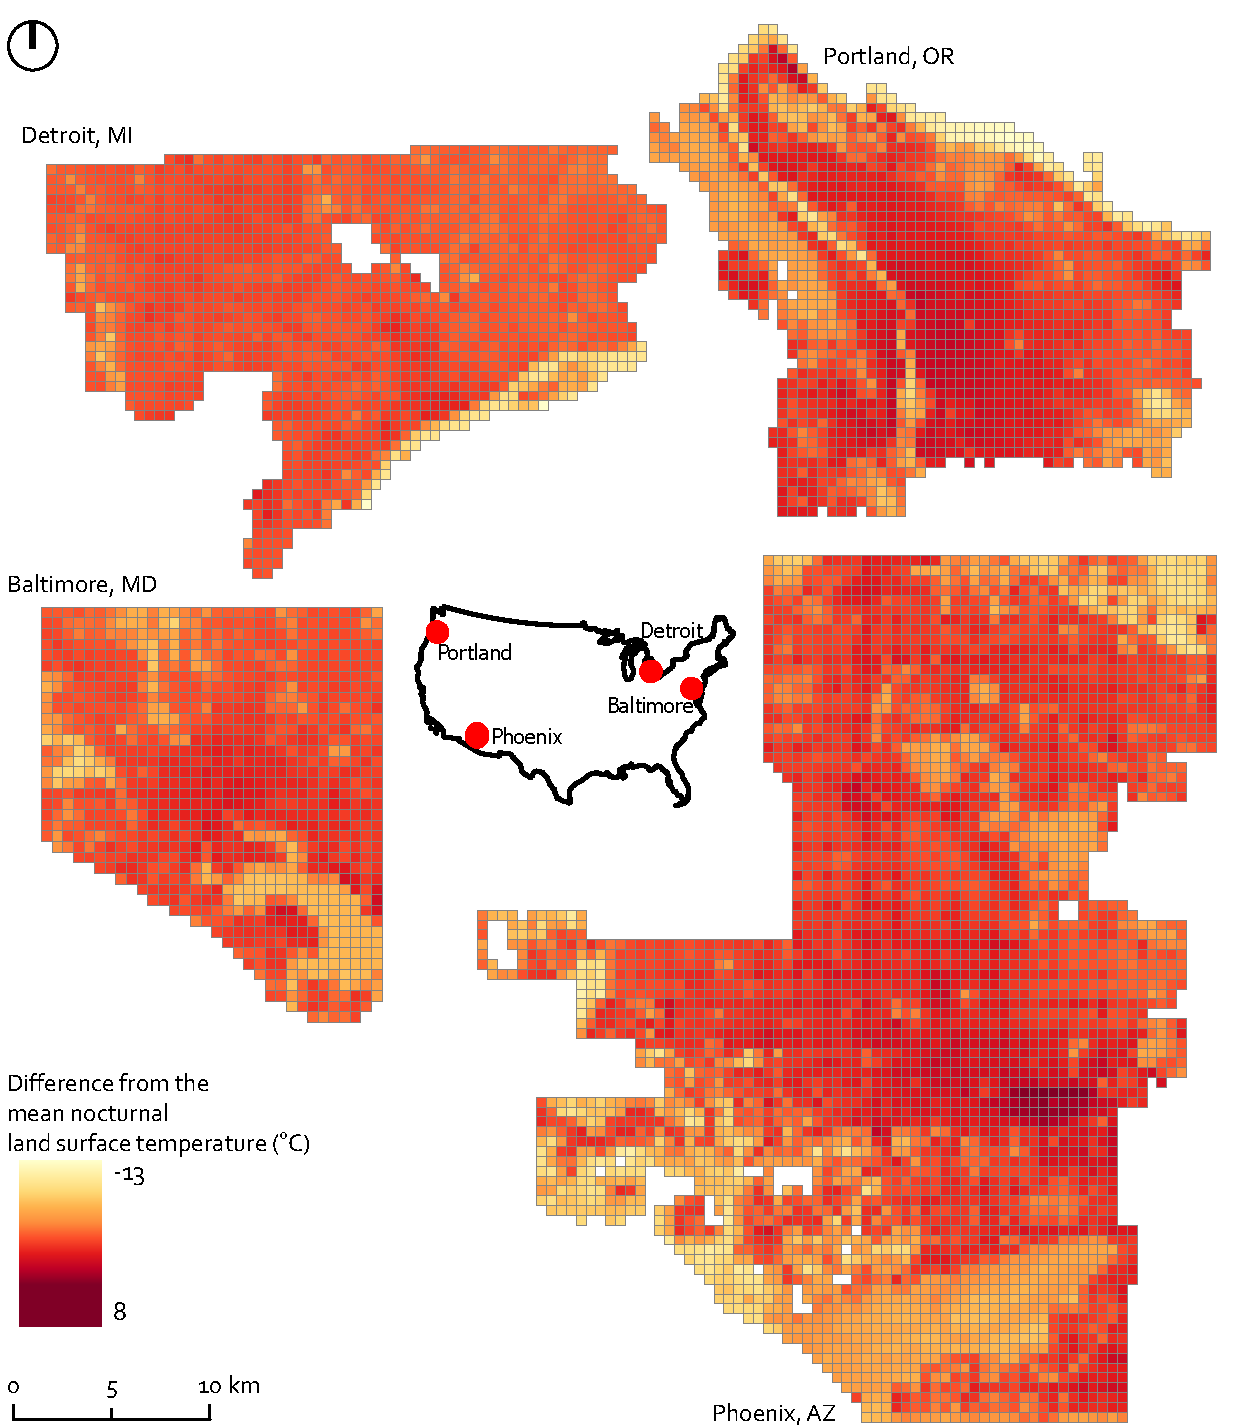
\includegraphics[width=\linewidth]{fig/report/map_nocturnal_lst.pdf}
    \caption{The gridded nocturnal land surface temperature in $^o$C of the cities studied. This is change from the mean (average) for each city.}
    \label{fig:map}
\end{figure}


\begin{figure}[H]
    \centering
    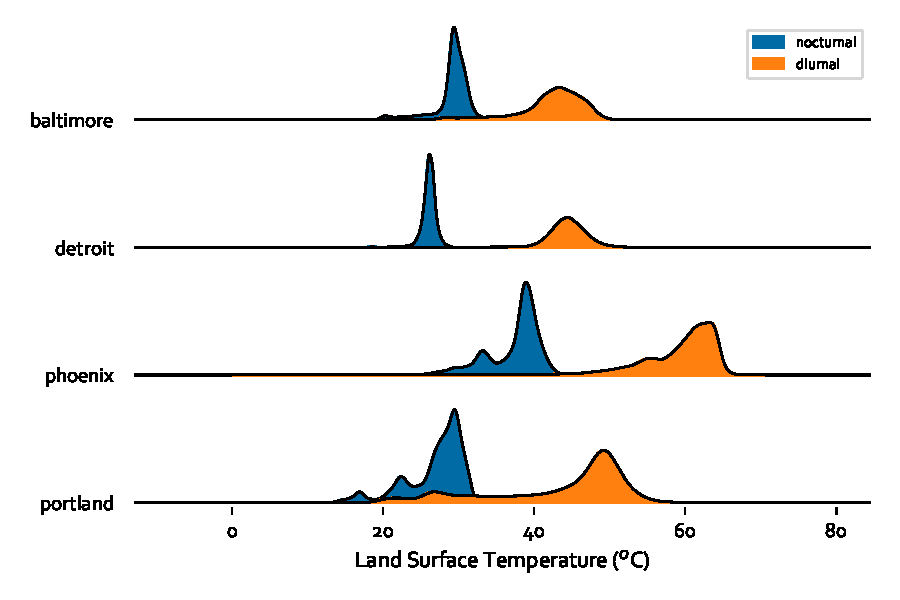
\includegraphics[width=\linewidth]{fig/report/joyplot_lst.pdf}
    \caption{The distribution of nocturnal and diurnal land surface temperature of the cities studied.}
    \label{fig:joy}
\end{figure}

\subsection{Land surface temperature}
We calculate land surface temperature using Landsat 8 (Land Processes Distributed Active Archive Center product) imagery as well as land cover and an air temperature observation (data sources provided in \ref{tab:data}. Band-10 digital-number data is converted to top-of-atmosphere radiance \cite{Jimenez-Munoz2003-wc}. We correct for emissivity using land cover data \cite{Alipour2003-gb}, and then calculate the at-satellite brightness temperature \cite{Jimenez-Munoz2003-wc}. Finally an atmospheric correction is made as per the monowindow algorithm \cite{Qin2001-jn} using the maximum observed temperature of the day from a nearby weather station. This follows the process is described in \cite{Scott2016-lc} and is explicitly outlined in our open source code on Github\footnote{URL redacted for review}. 

To ameliorate the effect of shadows and other ephemeral changes we use at least three minimal-cloud images for each city and night/day period and calculate the mean of LST.

- include scatter of night vs day LST at 100m - also change the symbols for colorblind - remove background
\begin{figure}[h]
\begin{center}
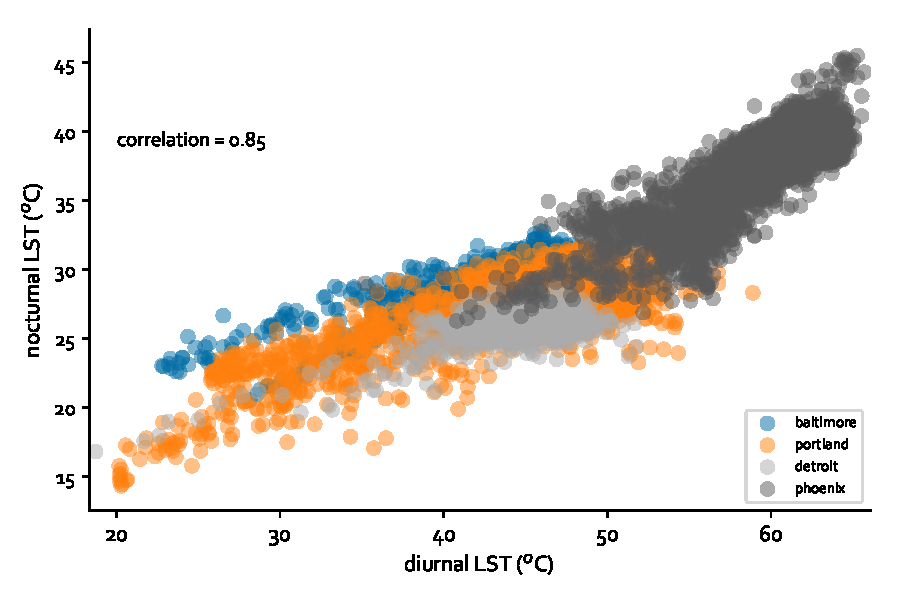
\includegraphics[width=\textwidth]{fig/report/lst_night-vs-day_500.pdf}
\caption{The land surface temperature in $^o$C of the cities studied at a 500m square resolution}
\label{fig:scatter_lst}
\end{center}
\end{figure}
\subsection{Independent variables}
- present correlation matrix of independent variables

\textit{Albedo}. Albedo is a measure of the reflectivity or brightness of a surface. It is normalized between 0-1 where the darker surfaces are lower values. Albedo is calculated using the LandSat8 images using the algorithm described in \cite{Smith2010-nw, Liang2001-jd}. 

\textit{Building floor area}. The building floor area within the cell. This uses data released in 2018 by Microsoft where building footprints are estimated using areal images. 

\textit{Building height}. Building height is estimated using the building footprints and available lidar data following \cite{Chun2017-mm}. The mean lidar elevation within each building's footprint is subtracted by the mean digital elevation (topography) within the footprint to estimate the building's height.

\textit{Elevation}. 1/3 arc-second (~10m) bare-earth elevation (topography) data is available courtesy the U.S. Geological Survey. The mean, max, and min of elevation points within the grid cell is calculated.

\textit{Surface elevation}. The surface elevation is determined from the lidar data. Surface elevation captures the natural and built features. 

\textit{Impervious surface percentage}. This is provided in the National Land Cover Database from the Multi-Resolution Land Charasteristic Consortium \cite{Xian2011-aa}. To generate the impervious surface area (ISA) LandSat data, NLCD land cover, and nighttime light imagery is used. The stable nighttime light intensity is only used to estimate the boundary of of urban areas. The Landsat images were converted to top-of-atmosphere reflectance. The data is provided at a 30m resolution and we calculate the mean, max, and min for each grid cell.

\textit{Land cover}. Classification of land cover is described in \cite{Homer2015-ce}. However, as it is used in the calculation of emissivity when calculating the LST it cannot be used as an independent variable. The only landcover that we use is category 11, water. Cells with more than 20\% area classified as water are excluded from the data set.

\textit{NBDI}. Normalized difference built-up index indicates the intensity of imperviousness \cite{Bhatti2014-ae}. It is calculated from satellite images as $$NDVI=\frac{B_{SWIR}-B_{NIR}}{B_{SWIR}+B_{NIR}}$$ where $B_{NIR}$ and $B_{SWIR}$ are the reflectances in the near-infrared and short-wave infrared bands respectively \cite{Alhawiti2016-wv}. Using LandSat8 imagery, this is $$NDVI=\frac{B6-B5}{B6+B5}$$ \cite{barsi2014}.
% *Kaplan 2018, Peng 2018

\textit{NDVI}. The normalized difference vegetation index (NDVI) measures green vegetation. It is calculated from satellite images as $$NDVI=\frac{B_{NIR}-B_{red}}{B_{NIR}+B_{red}}$$ where $B_{NIR}$ and $B_{red}$ are the reflectances in the near-infrared and red bands respectively \cite{Alhawiti2016-wv}. Using LandSat8 imagery, this is $$NDVI=\frac{B5-B4}{B5+B4}$$ \cite{barsi2014}.

\textit{Nighttime light intensity}. Stable nighttime light intensity is available from the Defense Meteorological Satellite Program (DMSP) Operational Linescan System (OLS). They prepare the data to remove clouds and ephemeral light sources. We use 2013 (the most recently available) data of version 4 at a spatial resolution of 30 arc-seconds (1km at the equator) \cite{ngdc2013version}. The nighttime light intensity was found to be only in moderate agreement with density \cite{bagan2018}, meaning lights may indicate anthropogenic energy use during the night. However, it's lower resolution means that can not capture minor differences. We resampled the raster to a 30m resolution, as per the NLDC \cite{Homer2015-ce}, and for each grid calculated the mean, min, and max.

\textit{Population density}. Density allegedly increases the LST \cite{Li2017-yl}, although this result may be the result of confounding with other factors. Population density calculated from the U.S. census at the block level. The most recent census was 2010, so that data is used as an estimator of where people reside in the evening. This data is also at a lower resolution that the grid cells used, so the grid cell assumes the density of the block that it's centroid is contained within.

\textit{Sky view factor}. Urban canyons have been found to have an effect on UHI because they prevent air circulation \cite{Landsberg1981, Chun2017-mm} and are used to indicate radiation flux within complex environments \cite{Matzarakis2007-xy}. We calculate SVF following using xxx and following the parameters used by \cite{Chun2017-mm}: the number of search directions, $\phi=10^o$; and the radius of the reference circle, $R=300m$. We use a spatial resolution of x-m.
% * Yuan 2011, Unger 2004.

\textit{Tree canopy cover}. The percent tree canopy cover is calculated using National Agriculture Imagery Program (NAIP) aerial imagery, Landsat 5 imagery, elevation, and existing NLCD data \cite{Coulston2012-uu, Homer2015-ce}. The data provided is at an xx resolution. The six reflective bands from Landsat 5 are used to calculate top-of-atmosphere reflectance \cite{Coulston2012-uu} so the product does not contain information used in the LST calculation (which requires radiance). 
% * Rogan 2013, Elmes 2017

\subsection{Statistical analysis}
The data was gridded into 500m square and 100m square cells for analysis. For each of the variables, the mean, maximum, and minimum were calculated. Spatially lagging, the mean of the surrounding cells (including diagonal) for each variable, was included as an additional independent variable to capture the spatial effects which may be present within the data. 
* test / train

* statistical models

\section{Results and Discussion}

\begin{figure}
    \centering
    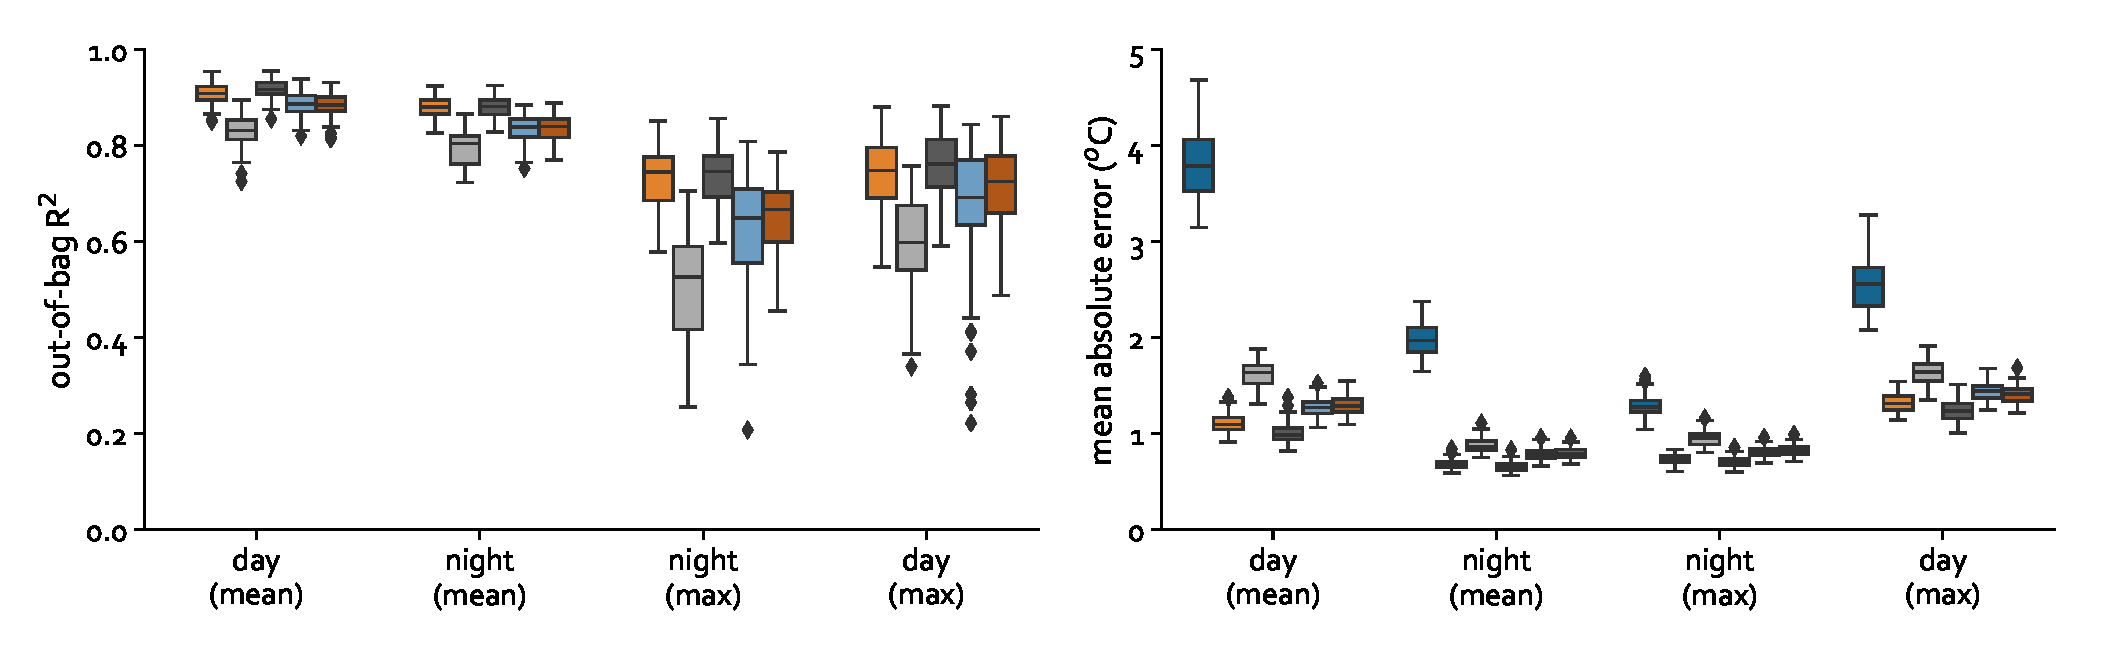
\includegraphics[width=\linewidth]{fig/report/holdout_results_500.pdf}
    \caption{
    The out-of-bag (OOB) R$^2$ and mean absolute error (MAE) of the models when fitted on three of the four cities and then used to predict the remaining city. OOB R$^2$ can vary between $(-\infty, 1)$, where better models have a value near 1. Good models have MAE near 0. The gradient boosted regression forest generally outperforms the other models, except when predicting Detroit. Note that the R$^2$ axis is truncated at -1, although the multiple linear regression for diurnal land surface temperature tested on Phoenix has an OOB R$^2$ of -9.  This shows that the gradient boosted regression forest (gbm) consistently outperforms the multiple linear regression and null models.
    }
    \label{fig:holdout_results}
\end{figure}

\subsection{Variables related to Land Surface Temperature}

\begin{figure}
    \centering
    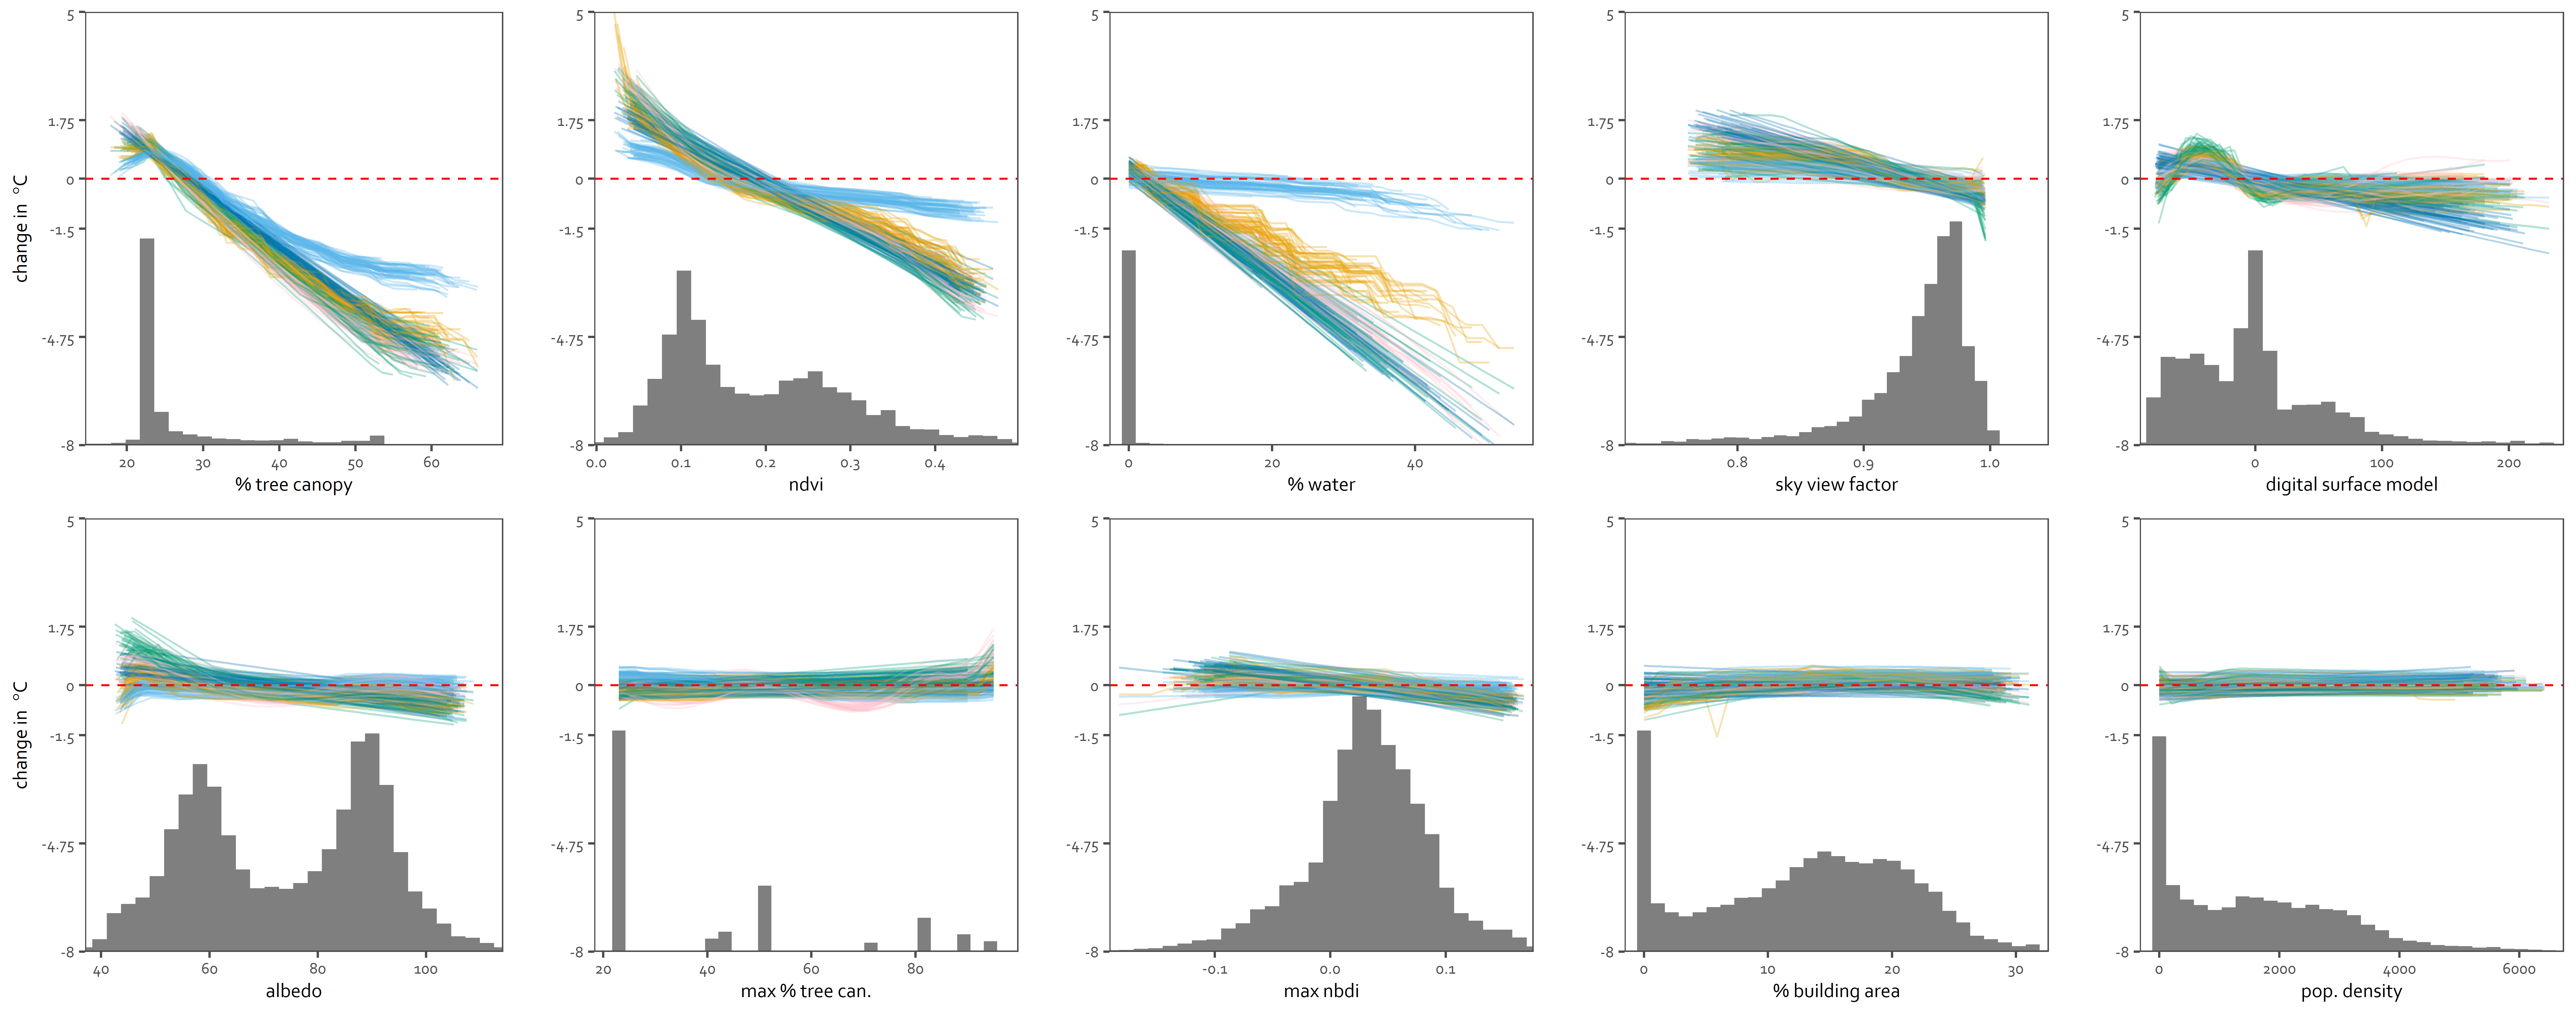
\includegraphics[width=\linewidth]{fig/report/pdp_uncert_night.png}
    \caption{
    Partial dependence plots show how the land surface temperature ($^oC$, y axis) changes with each variable as the other variables are held at their average value. The left hand side shows the effect each variable has on LST during the night, while the right hand side shows the effect during the day. This shows that trees coverage in the cell has the greatest influence on the temperature, and the greenness (NDVI) of that coverage matters during the day.
    }
    \label{fig:pdp_night}
\end{figure}

\begin{figure}
    \centering
    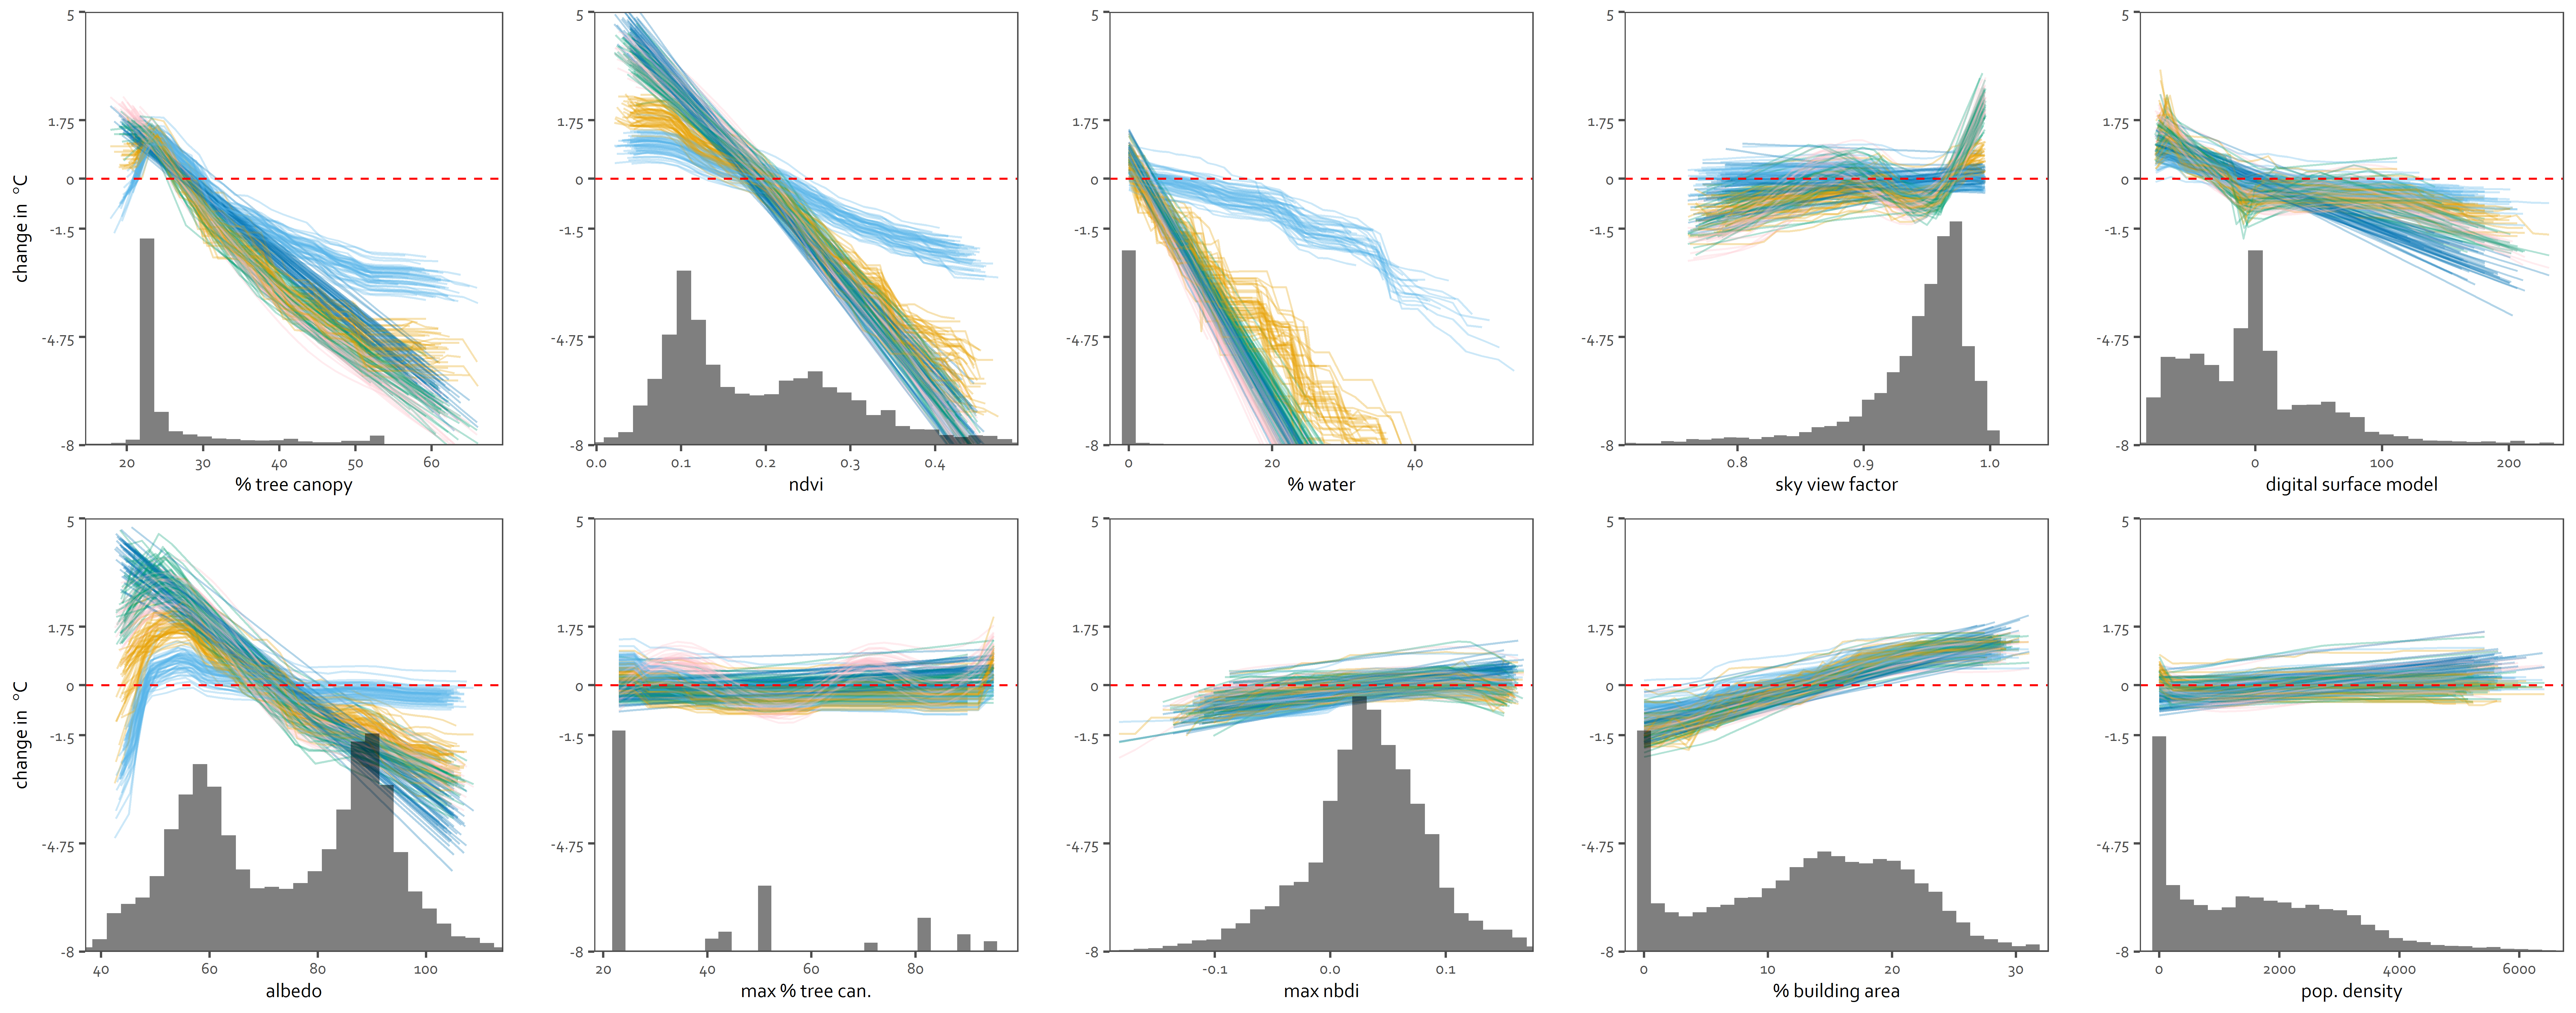
\includegraphics[width=\linewidth]{fig/report/pdp_uncert_day.png}
    \caption{
    Partial dependence plots show how the land surface temperature ($^oC$, y axis) changes with each variable as the other variables are held at their average value. The left hand side shows the effect each variable has on LST during the night, while the right hand side shows the effect during the day. This shows that trees coverage in the cell has the greatest influence on the temperature, and the greenness (NDVI) of that coverage matters during the day.
    }
    \label{fig:pdp_day}
\end{figure}



\section{Drivers of LST}
See figure \ref{fig:importance} and \ref{fig:pdp}.

Regarding Fig \ref{fig:pdp}, I think I will remove the ``all" line, because in cases such as $alb_mean_min_sl$ (which is the minimum albedo in the surrounding cells (sl = spatial lag)) the values between the cities don't overlap so I think it becomes a proxy for other differences between the city when regressed together.

\begin{figure}[h]
\begin{center}
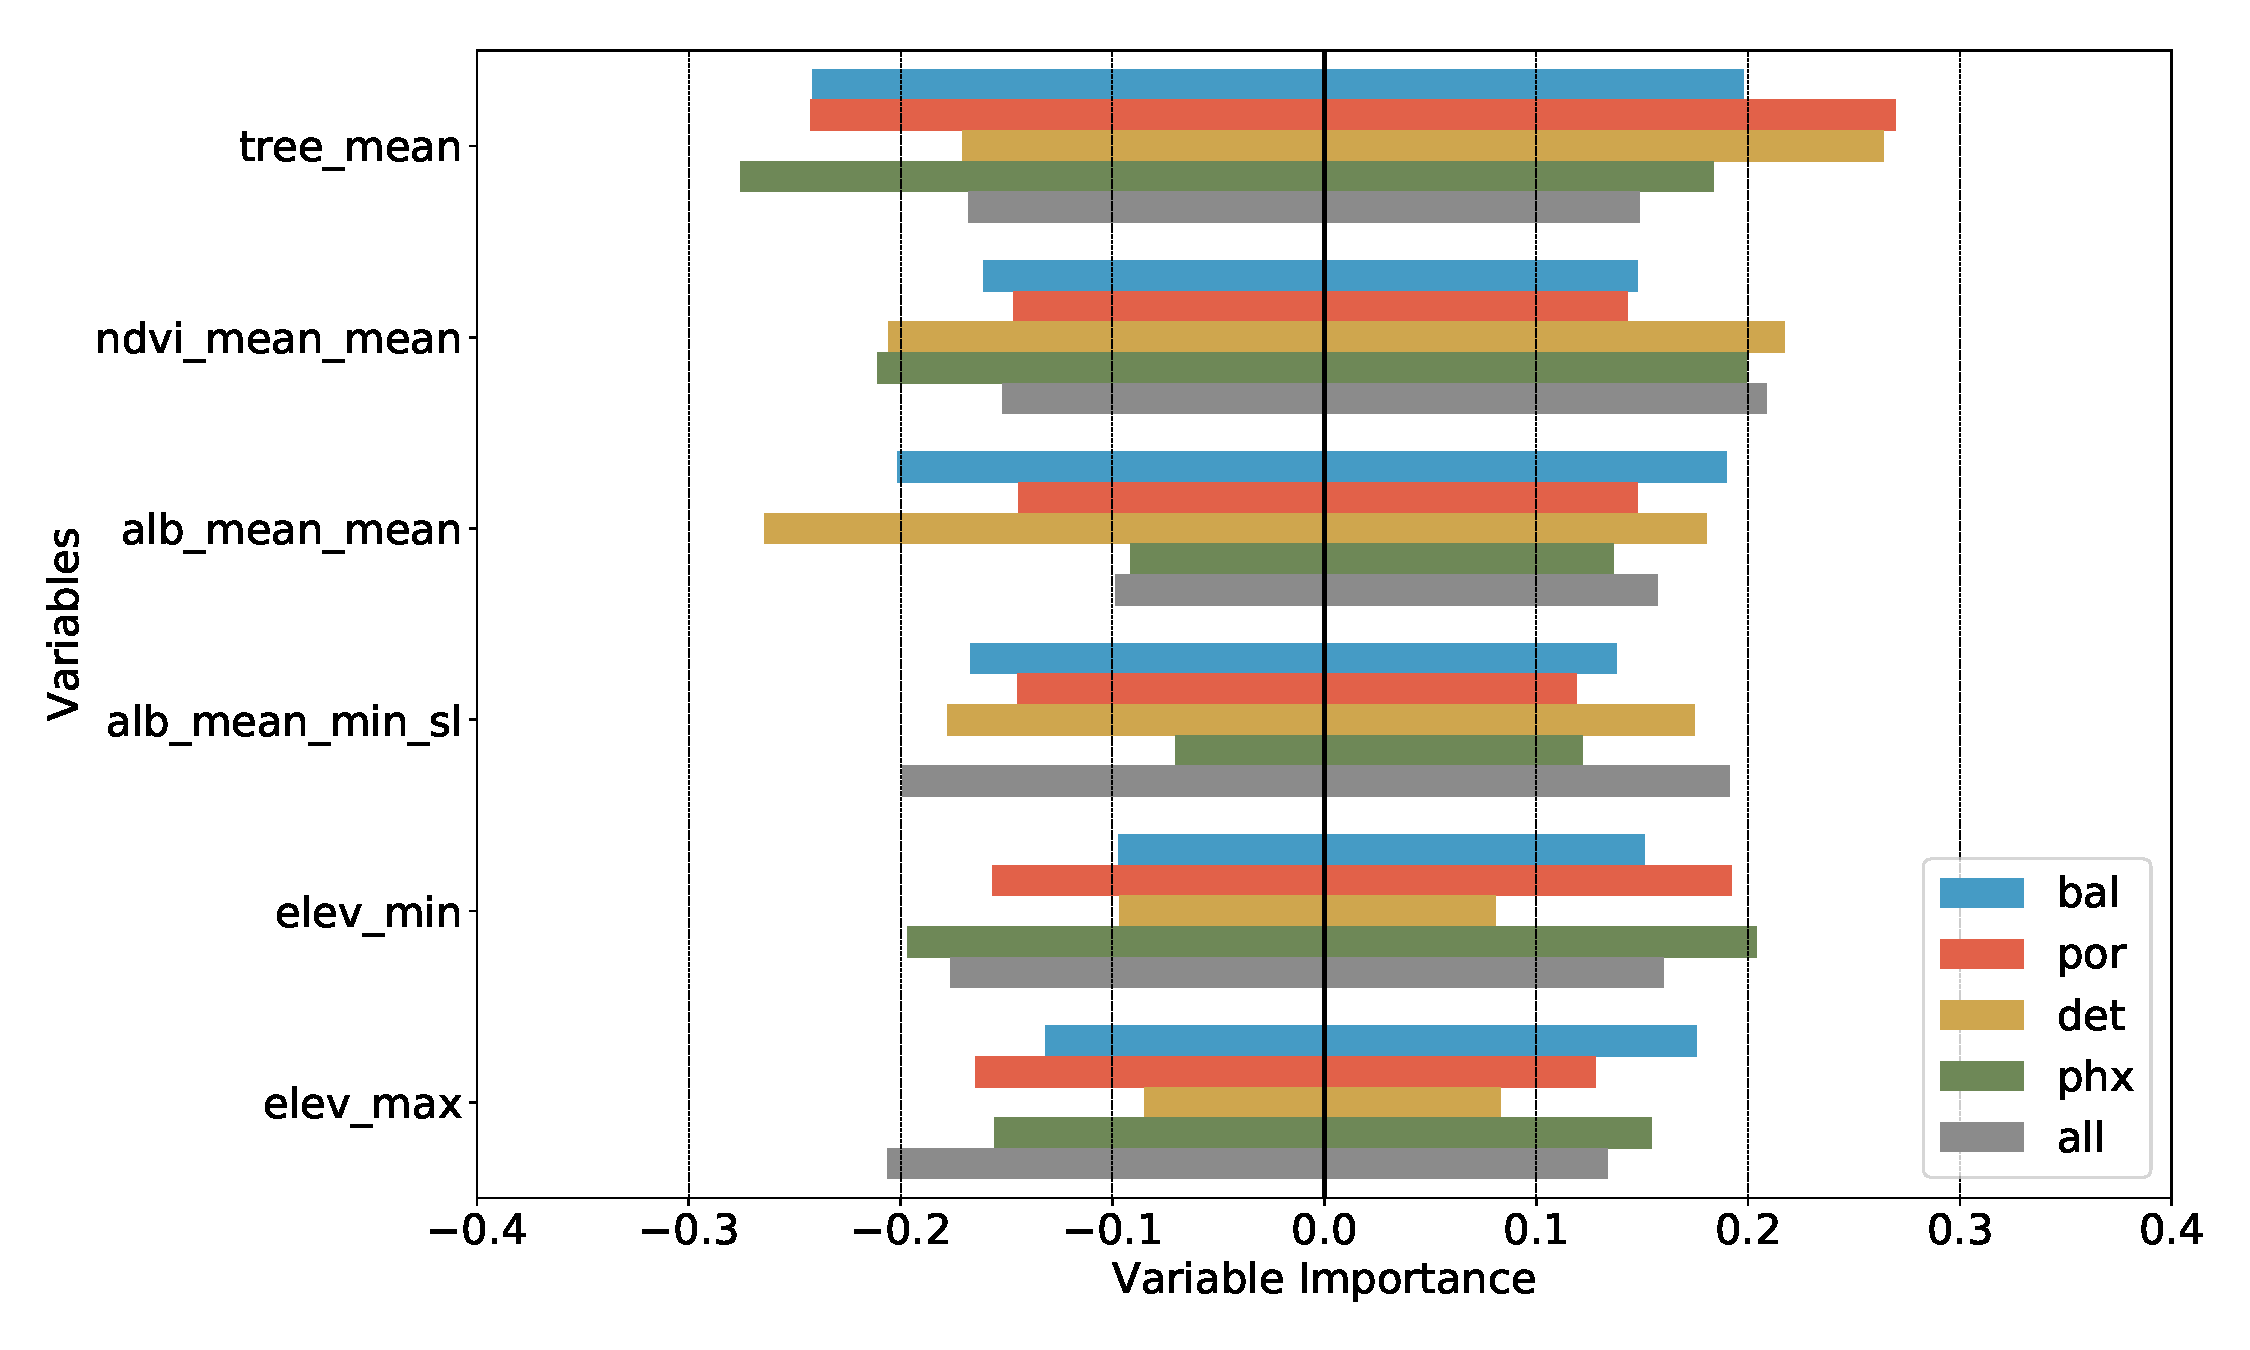
\includegraphics[width=\textwidth]{fig/report/variable_importance_selected.pdf}
\caption{The variable importance for the regression during the night (to the left) and the day (to the right). Variable importance indicates the amount that each variable improves the performance of the regression.
In this case there is generally little difference between the importance of day and night variables.}
\label{fig:importance}
\end{center}
\end{figure}

\begin{figure}[h]
\begin{center}
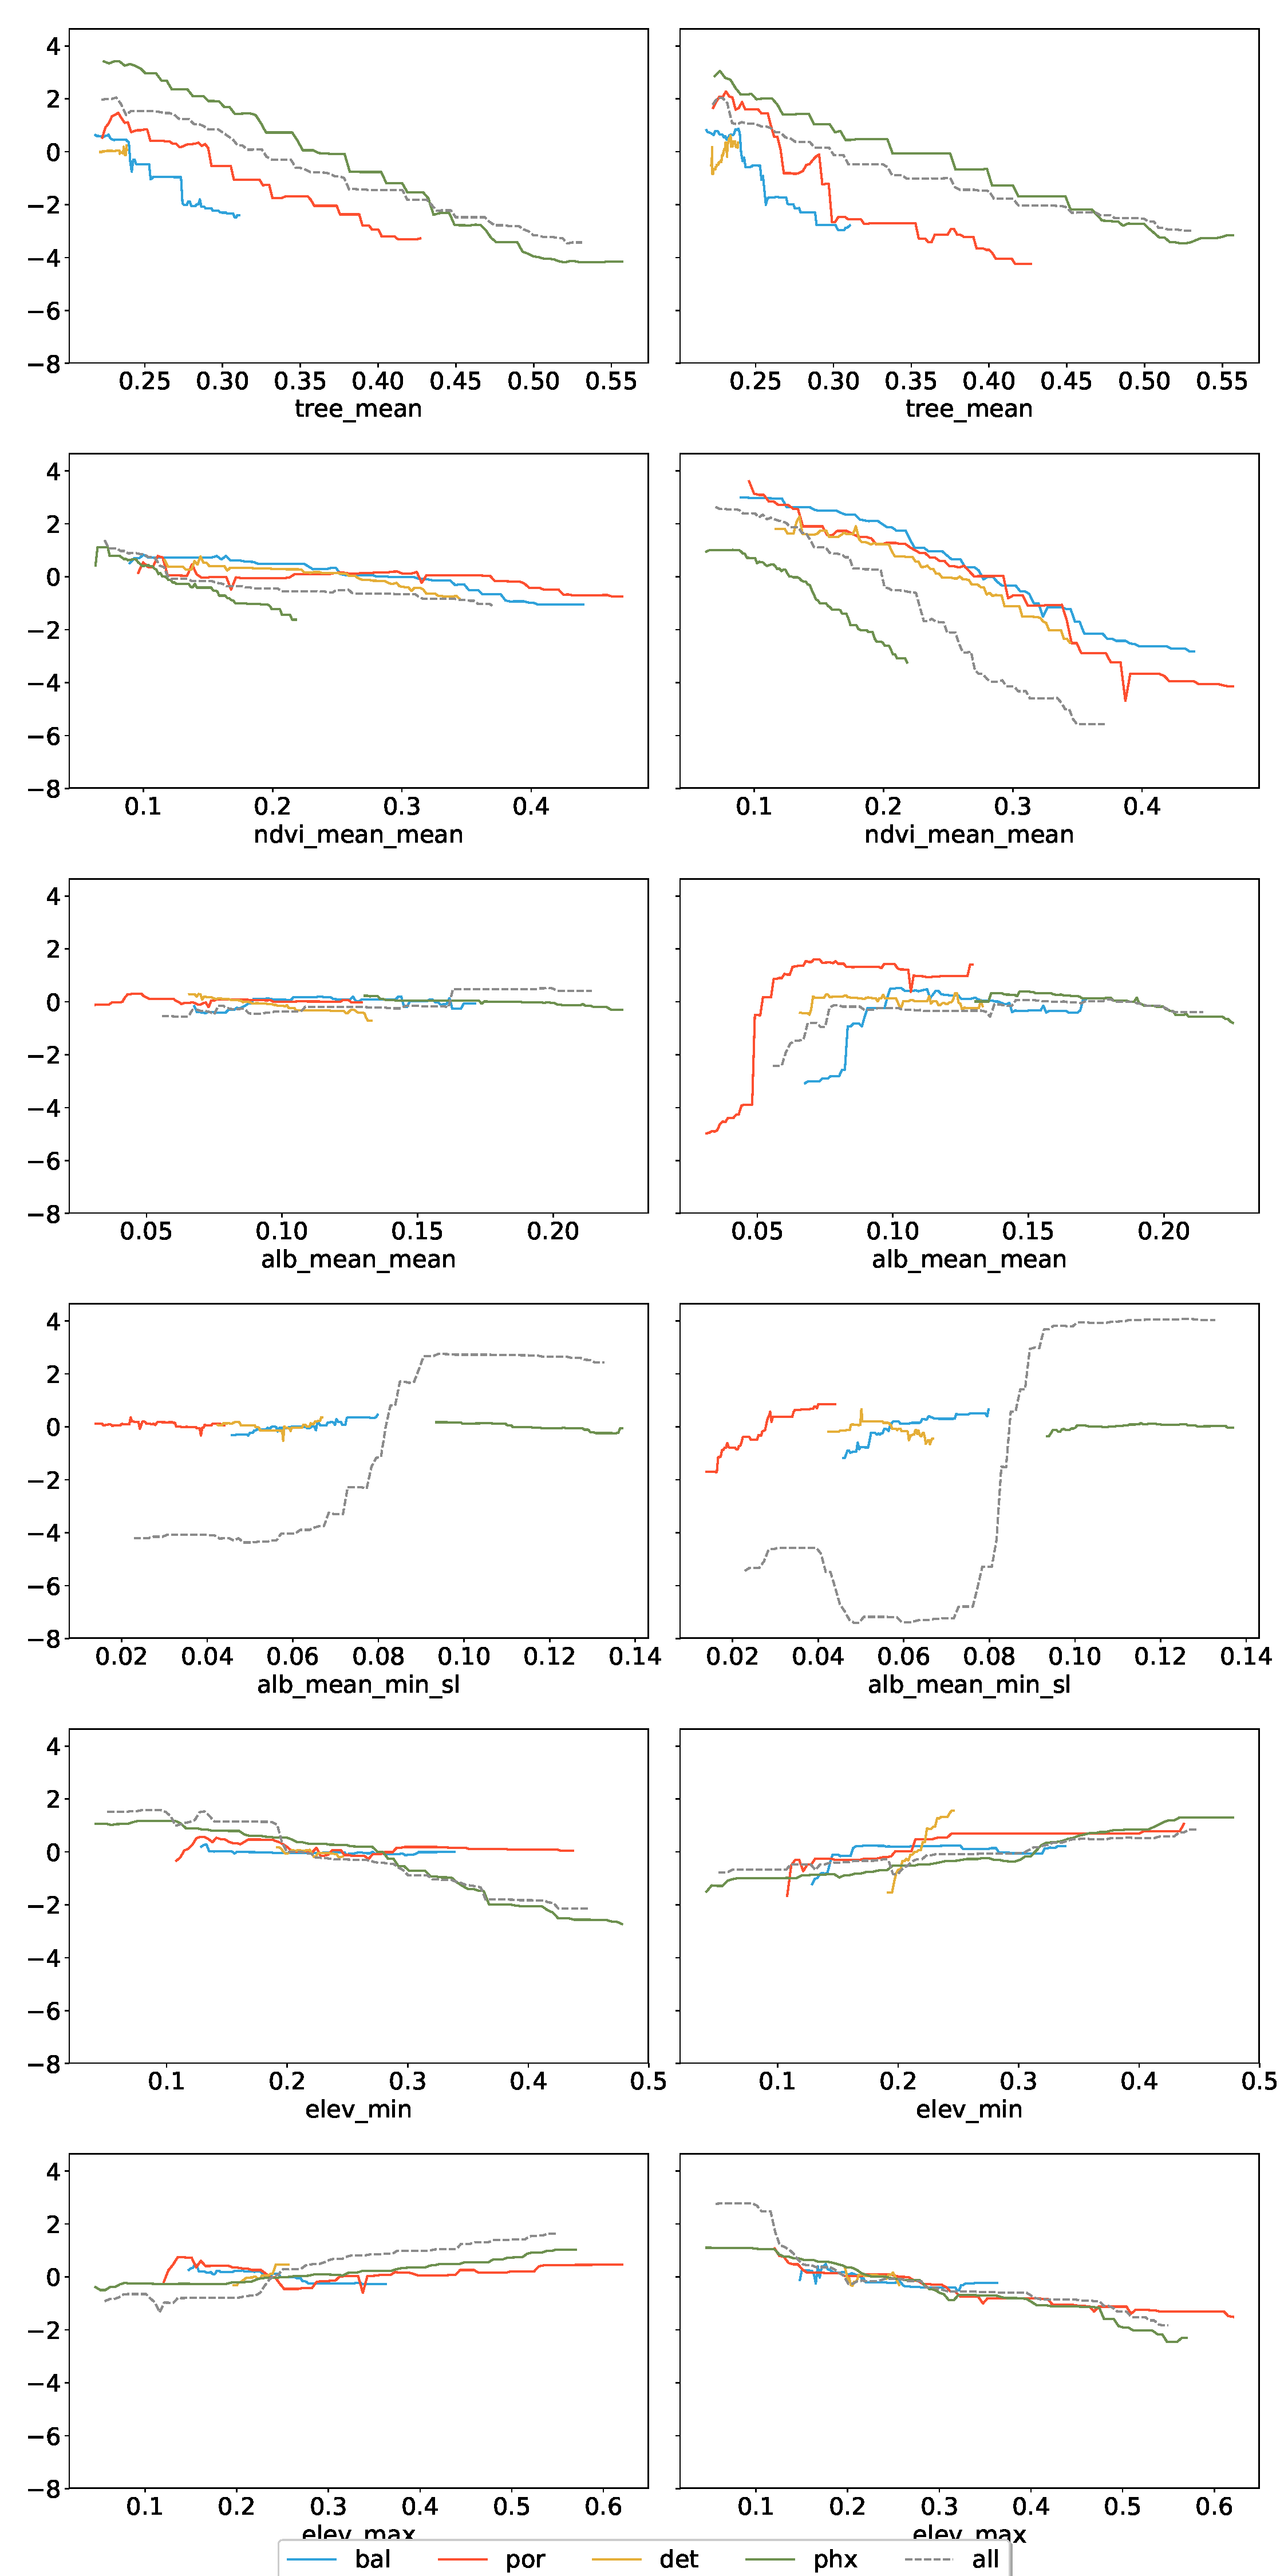
\includegraphics[height=\textheight]{fig/report/partial_dependence.pdf}
\caption{Partial dependence plots show how the land surface temperature ($^oC$, y axis) changes with each variable as the other variables are held at their average value. The left hand side shows the effect each variable has on LST during the night, while the right hand side shows the effect during the day. This shows that trees coverage in the cell has the greatest influence on the temperature, and the greenness (NDVI) of that coverage matters during the day.}
\label{fig:pdp}
\end{center}
\end{figure}



% \section{Conclusion}

% There are various bibliography styles available. You can select the style of your choice in the preamble of this document. These styles are Elsevier styles based on standard styles like Harvard and Vancouver. Please use Bib\TeX\ to generate your bibliography and include DOIs whenever available.

% Here are two sample references: \cite{Feynman1963118,Dirac1953888}.

\section*{References}

\bibliography{mybibfile}

\appendix
\section{Data sources}

\begin{tabu}to \textwidth{ X[l]  X[c]  X[c] X[l] X[l] }
 \hline
 Data Provider & Data Type & Data Date & Description & URL \\
 \hline
U.S. Geological Survey  & Raster  & 2013-2017 &
    Landsat 8 day and night satellite imagery & \burl{https://earthexplorer.usgs.gov/} \\
Microsoft  & Polygon  & 2018 & Building footprint polygons for the US &
    \burl{https://github.com/Microsoft/USBuildingFootprints} \\
Defense Meteorological Satellite Program  & Raster  & 2013 &
    Stable nighttime light intensity & \burl{https://www.ngdc.noaa.gov/eog/dmsp/downloadV4composites.html} \\
Multi-Resolution Land Characteristics Consortium  & Raster  & 2011 &
    Land cover & \burl{https://www.mrlc.gov} \\
Multi-Resolution Land Characteristics Consortium  & Raster  & 2011 &
    Percent developed imperviousness & \burl{https://viewer.nationalmap.gov} \\
Multi-Resolution Land Characteristics Consortium  & Raster  & 2011 &
    Percent tree canopy cover & \burl{https://viewer.nationalmap.gov} \\
U.S. Geological Survey  & Raster  & 2015 & 1/3 arc-second elevation &
    \burl{https://nationalmap.gov/3DEP/3dep_prodserv.html} \\
U.S. National Oceanic and Atmospheric Administration  & Lidar  & 2014 & Point cloud of surface elevation &
    \burl{https://coast.noaa.gov/htdata/lidar2_z/geoid12b/data/6377/} \\
IPUMS NHGIS  & Area Level  & 2010 &
    Block-level population from the US census & \cite{nhgis}\\
\hline
\label{tab:data}
\end{tabu}




\section{Additional model results}
\begin{figure}[h]
\begin{center}
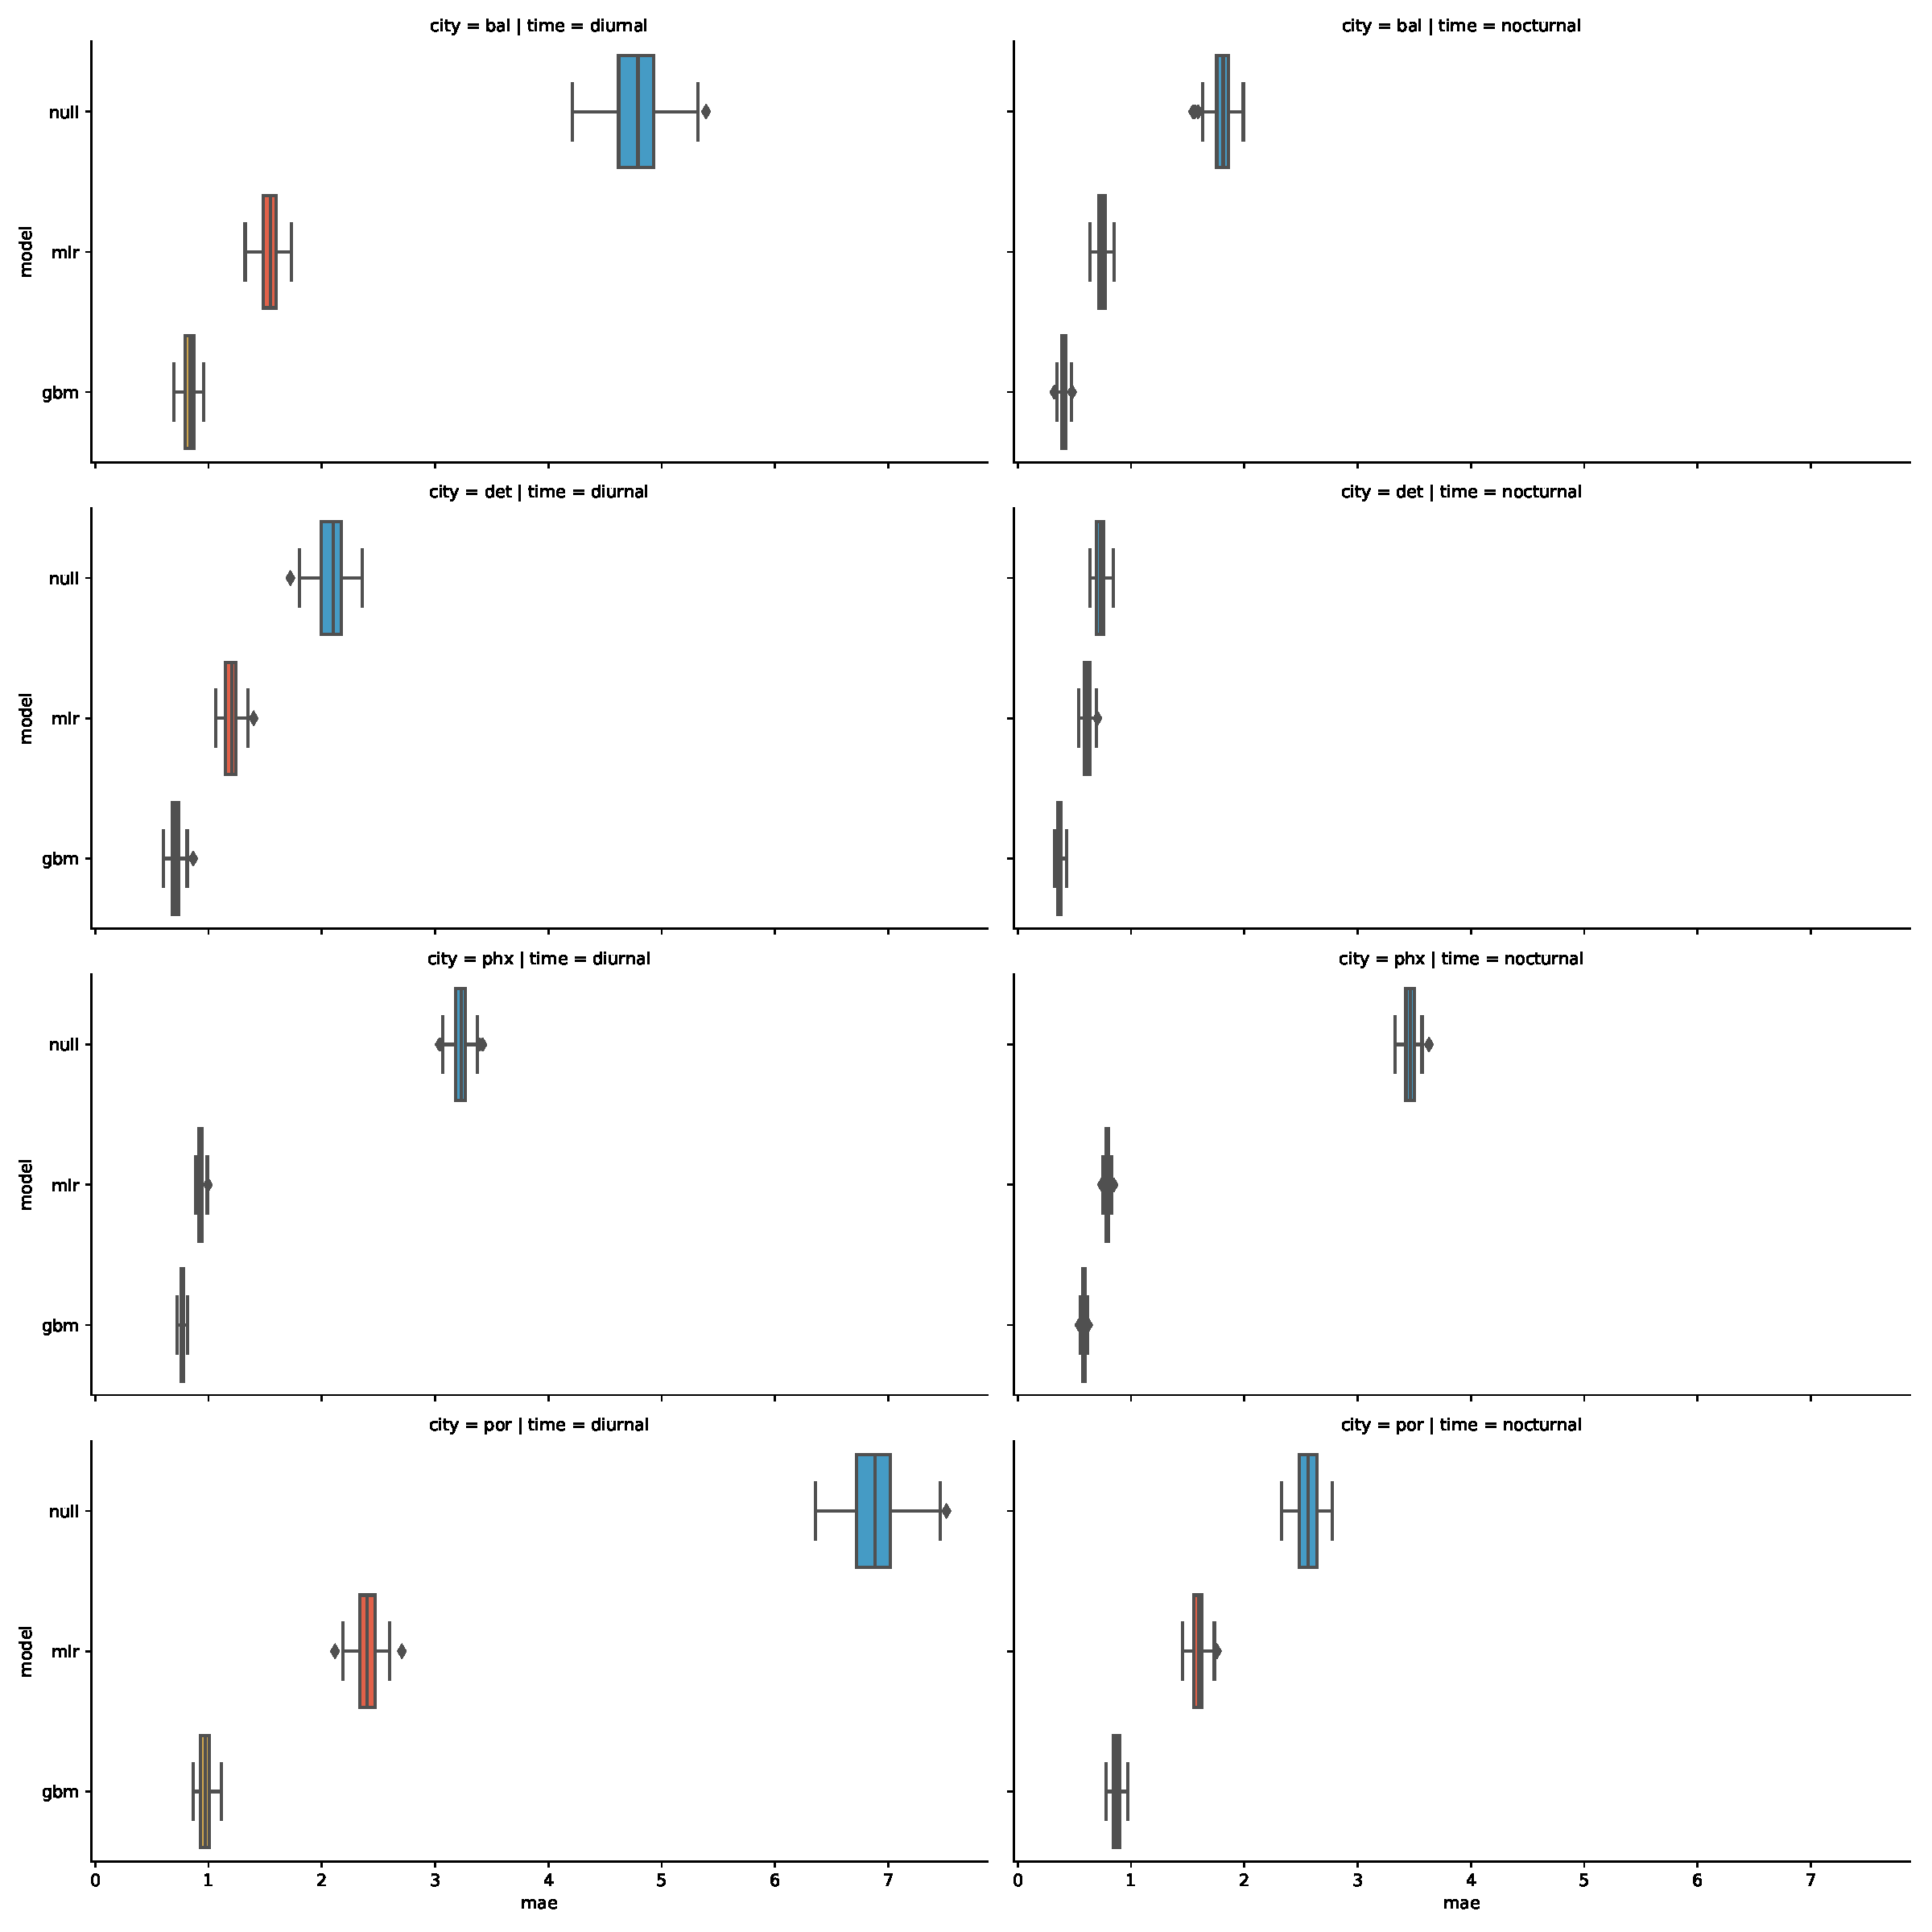
\includegraphics[width=\textwidth]{fig/report/holdout_results_mae.pdf}
\caption{The Mean Absolute Error (MAE) in $^oC$ of the models when fitted on each city and used to predict a random sample from the same city. Better models have lower MAE. This shows that the gradient boosted regression forest (gbm) consistently outperforms the multiple linear regression and null models. }
\label{fig:cityholdout_errors}
\end{center}
\end{figure}




\end{document}
